\documentclass[a4paper, 12 pt]{article}

\usepackage{graphicx, float}
\usepackage{fourier}
\usepackage[french]{babel}
\usepackage[T1]{fontenc}
\usepackage[utf8]{inputenc}

\title{\LARGE \textbf{LES VUES MULTIPLES D'UN SOLIDE}}
\author{MATH\'EMATHIQUES 5P}
\date{\today}



\begin{document}

    \Large
    

    \begin{titlepage}
        
        \maketitle
    \end{titlepage}
    
    \setcounter{page}{2}

    %\tableofcontents

    %\newpage

    \section{Vue de gauche}

        \begin{figure}[H]
            \centering
            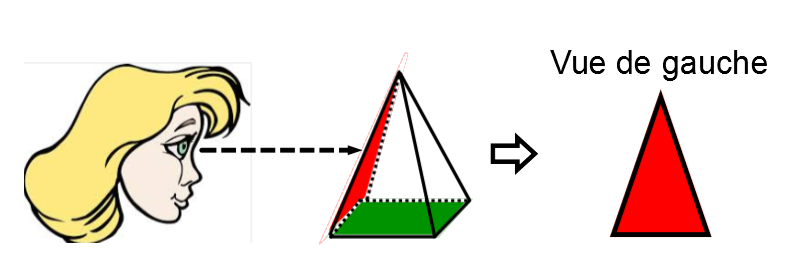
\includegraphics[width = 1\linewidth]{img\vueGauche.PNG}
            \caption[]{Visualiser le solide depuis la gauche}
        \end{figure}

    
    Exercices :

   \newpage
   \section{Vues coordonnées}
   Ci-dessous, on a les vues de face, de haut et de gauche de la pyramide
        \begin{figure}[H]
            \centering
            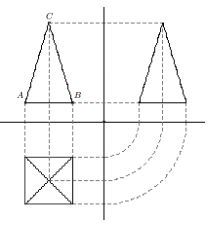
\includegraphics[width = 1\linewidth]{img\coordo.PNG}
            \caption[]{Visualiser le solide depuis le haut}
        \end{figure}

    Exercices :\begin{itemize}
        \item Représente les vues de face, de haut, de gauche et de droite de la pyramide L8 P6 H7
        \item Représente les vues demandées ci-dessous: \begin{figure}[H]
            \centering
            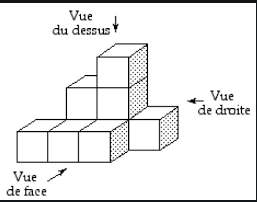
\includegraphics[width = 1\linewidth]{img\cubes.PNG}
            \caption[]{Visualiser le solide depuis le haut}
        \end{figure}
        
    \end{itemize}
    Représente les vues de face, de haut, de gauche et de droite de la pyramide L8 P6 H7
    
\end{document}
